\section{Paper 2}
\subsection{\emph{"Linear Spectral Clustering Superpixel"}}
\begin{frame}{INTRODUCTION}
    The introduced technique is called SUPERPIXEL. Widely used in image 
    processing for particular tasks such as image segmentation, image analysis, 
    image classification, target tracking, 3D reconstruction, surface retrieval and 
    object proposal. The purpose of the elaborate story is to reduce the 
    computational complexity through a superpixel system called LSC (Linear Spectral
    Clustering).
\end{frame}

\begin{frame}{LSC SUPERPIXEL pt1}
    Goal: optimization (max/min) of two objective functions to create clusters of pixels called superpixels:
    \begin{block}{Objective Function 1: Weighted K-Means}
        $$ F_{km} = \sum_{k=1}^K\sum_{p\in\pi_k}\omega(p)= || \phi(p)-m_k ||^2 $$
    \end{block}
    \begin{block}{Objective Function 2: Normalized cuts}
        $$ F_{N_{cuts}} = \frac{1}{K}\sum_{k=1}^K\frac{\sum_{p\in\pi_k}\sum_{q\in\pi_k}W(p,q)}{\sum_{p\in\pi_k}\sum_{q\in{V}}W(p,q)} $$
    \end{block}
    Problem: extremely high computational!
\end{frame}

\begin{frame}{LSC SUPERPIXEL pt2}
    If corollary 1 is satisfied, then  \emph{weghted K-means clustering} can be used 
    for segmentation and for creation of superpixel regions, instead of the 
    eigen-vector based method.
    \begin{block}{\bfseries{Corollary 1}}
        Optimizations of the objective functions of the weighted K-means
        and the normalized cuts are mathematically equivalent if (1) and (2) 
        hold simultaneously. The symbol $ \cdot $ stands for inner product.
    \end{block}

    \begin{block}{Equation (1)}
           $$ \omega(p)\phi(p) \cdot \omega(q)\phi(q) = W(p,q), \forall p,q \in V $$
    \end{block}

    \begin{block}{Equation (2)}
        $$ \omega(p) = \sum_{q \in V} W(p,q), \forall p \in V $$
    \end{block}
\end{frame}

\begin{frame}{LSC Algorithm pt1}
    Problem? $ \rightarrow $ Find the correct positive similarity function $ W (p,q) $, 
    between two data points \emph{p} and \emph{q} to solve equation 1.
    \begin{block}{Similarity Function}
        \begin{equation}\small
            \begin{split}
                W(p,q) = C_s^2(\cos \frac{\pi}{2}(x_p-x_q)+\cos\frac{\pi}{2}(y_p-y_q)) \\
                + C_c^2(\cos \frac{\pi}{2}(l_p-l_q)+\cos\frac{\pi}{2}(\alpha_p-\alpha_q) \\
                + \cos\frac{\pi}{2}(\beta_p-\beta_q)x2.55^2)
            \end{split}
        \end{equation}
    \end{block}
    
    \begin{block}{Mapping Function}
        \begin{equation}\small
            \begin{split}
                \phi(p) = \frac{1}{\omega(p)}[C_c\cos\frac{\pi}{2}l_p, C_c\sin\frac{\pi}{2}l_p, 2.55C_c\cos\frac{\pi}{2}\alpha_p \\
                x 2.55C_c\sin\frac{\pi}{2}\alpha_p, 2.55C_c\cos\frac{\pi}{2}\beta_p, 2.55C_c\sin\frac{\pi}{2}\alpha_p, \\
                x C_s\cos\frac{\pi}{2}x_p, C_s\sin\frac{\pi}{2}x_p, C_s\cos\frac{\pi}{2}y_p, C_s\sin\frac{\pi}{2}x_p]
            \end{split}
        \end{equation} 
    \end{block}
    
\end{frame}

\begin{frame}{LSC Algorithm pt2}
    Assuming that equation 1 exists, LSC method takes two parameters as 
    input; The image to be segmented and the preferred K number of 
    superpixels that the algorithm will have to produce. The number K 
    corresponds to the number of centroids and each of these will be useful 
    for grouping the neighbors pixels, in a range of $ \tau v_x \ x \ \tau v_y $, with $ \tau>0.5 $, 
    using a distance comparison.
    \begin{figure}[h!]
        \centering
        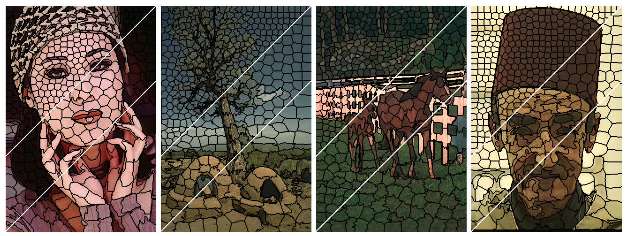
\includegraphics[width = 0.7 \linewidth]{paper2/slide1.png}
        \centering
        \caption{Sample images segmented with K = 1000/500/200 superpixels using LSC.}
        \label{fig: metrics}
    \end{figure}
\end{frame}

\begin{frame}{COMPARATIVE EXPERIMENTS}
    \begin{table}[htbp!]
        \centering
        \begin{adjustbox}{max width=\textwidth}
        \begin{tabular}{*{9}{|c}|}%%{|c|c|c|c|c|c|c|c|c|}
            \hline
            & EneOpt0 & SEEDS\footfullcite{0781426509} & ERS\footfullcite{0781426508} & Lattices & NCuts & SLIC\footfullcite{0781426514} & Turbo & LSC \\
            \hline
            \bfseries{ADERENCE TO BOUNDARY} & & & & & & & & \\
            \emph{Under segmentation error} & 0.230 & 0.197 & 0.198 & 0.303 & 0.220 & 0.213 & 0.277 & \bfseries{0.190}\\
            \emph{Boundary recall} & 0.765 & 0.918 & 0.920 & 0.811 & 0.789 & 0.837 & 0.739 & \bfseries{0.926}\\
            \emph{Achievable segmentation accuracy} & 0.950 & 0.960 & 0.959 & 0.933 & 0.956 & 0.956 & 0.943 & \bfseries{0.962}\\
            \hline
            \bfseries{SEGMENTATION SPEED} & & & & & & & & \\
            \emph{Computational complexity} & $ O(N^3/K^2) $ & $ O(N) $ & $ O(N^2 \lg{N}) $ & $ O(N^{\frac{3}{2}} \lg{N}) $ & $ O(N^{\frac{3}{2}}) $ & $ O(N) $ & $ O(N) $ & $ O(N) $\\
            \emph{Average time per image} & 3.35s & \bfseries{0.0935}s & 0.969s & 0.284s & 93.4s & 0.125s & 6.61s & 0.334s\\
            \hline
        \end{tabular}
        \end{adjustbox}
        \caption{Performance metrics superpixel segmentation algorithms at K=400}
        \label{table superpixels}
    \end{table}
    Best performance: low "Under segmentation Error" (\emph{UE}), high 
    "Boundary Recall" (\emph{BR}) and high "Achievable segmentation accuracy 
    (\emph{ASA}).
\end{frame}

\begin{frame}{APPLICATIONS: Class segmentation}
    \begin{figure}[htbp]
        \centering
        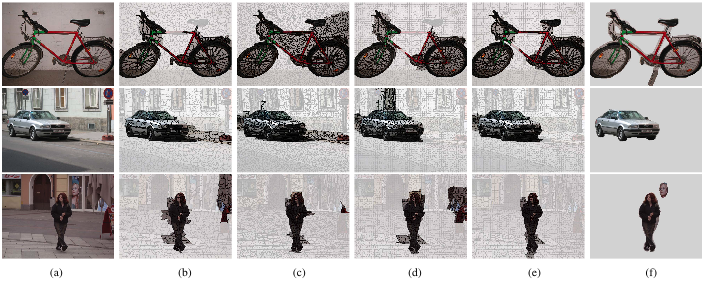
\includegraphics[width = 1 \linewidth]{images/paper2/superpixelAlgo.png}
        \centering
        \caption{Segmentation using different superpixels algorithms. (a) Original Image. (b) QS. (c) ERS. (d) SLIC. (e) LSC. (f)Ground Truth.}
        \label{fig: superpixelSegmentation}
    \end{figure}

    \begin{table}[h!]
        \centering
        \begin{adjustbox}{max width=4cm}
        \begin{tabular}{*{5}{|c}|}%%{|c|c|c|c|c|}
            \hline
            & QS & ERS & SLIC & LSC\\
            \hline
            bike & 72.2 & 74.2 & 76.3 & \bfseries{76.9}\\
            cars & 72.2 & 74.7 & 72.5 & \bfseries{76.8}\\
            person & 66.3 & 66.5 & 66.7 & \bfseries{67.0}\\
            \hline
        \end{tabular}
        \end{adjustbox}
        \caption{Accuracy using different superpixels algorithms.}
        \label{table accuracy}
    \end{table}
\end{frame}

\begin{frame}{APPLICATIONS: Weakly Supervised Semantic Segmentation}
    \begin{minipage}{\linewidth}
        \centering
        \begin{minipage}{0.45\linewidth}
            \begin{figure}[H]
                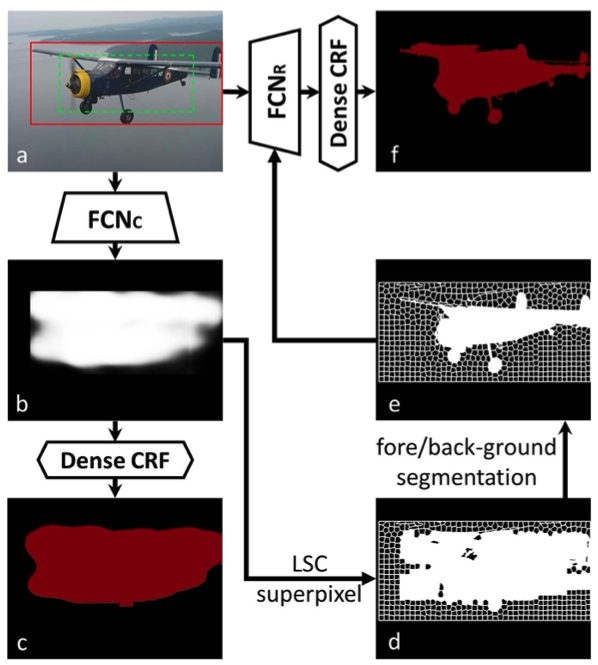
\includegraphics[width = 0.7 \linewidth]{images/paper2/semanticSegmentation.png}
                \caption{Weakly supervised semantic segmentation. (a) A training image with bounding boxes. (b) Output of soft-max layer of $ FCN_c $. (c) Coarse semantic segmentation result. (d) Superpixels with higher probability of foreground. (e) Fore-/Background segmentation result after iterative optimization. (f) Refined semantic segmentation result.}
            \end{figure}
        \end{minipage}
        \hspace{0.05\linewidth}
        \begin{minipage}{0.45\linewidth}
            \begin{figure}[htbp]
                \centering
                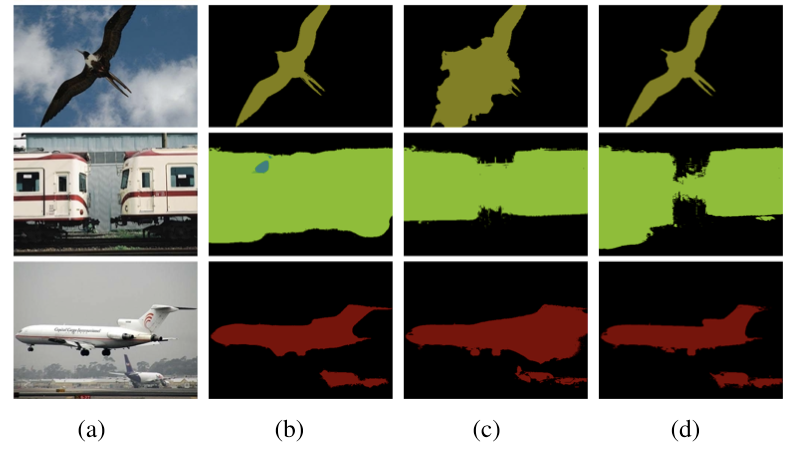
\includegraphics[width = 1 \linewidth]{images/paper2/segmentationAlgo.png}
                \centering
                \caption{Semantic segmentation. (a) Input image. (b) Strong. (c) Bbox-seg. (d) $ Joint_{sp} $ (LSC) }
            \end{figure}
            \begin{table}[H]
                \begin{adjustbox}{max width=4cm}
                    \begin{tabular}{*{3}{|c}|}%%{|c|c|c|}
                        \hline
                        Strong\footnotemark[1]& Bbox-seg\footnotemark[1] & $ Joint_{sp} $ \\
                        \hline
                        62.5 & 60.6 & \bfseries{64.0} \\
                        \hline
                    \end{tabular}
                \end{adjustbox}
                \caption{Semantic segmentation accuracy in terms of Mean IOU (\%)}
            \end{table}
        \end{minipage}
    \end{minipage}
    \footnotetext[1]{\tiny G. Papandreou, L. Chen, K. Murphy, and A. Yuille, “Weakly-and semi-
    supervised learning of a deep convolutional network for semantic image segmentation,” in Proc. ICCV, pp. 1742–1750, Dec. 2015}
\end{frame}

\begin{frame}{CONCLUSIONS}
    The LSC algorithm seems to be the best in terms of adherence to the 
    boundary and in the creation of superpixels with increasingly regular 
    shape, but there are still two problems to solve:
    \begin{enumerate}
        \item The number K of superpixels entered manually
        \item New similarity techniques to improve performance
    \end{enumerate}
\end{frame}